\begin{minipage}[b]{0.33\linewidth}
\begin{lrbox}{\mybox}%
\begin{lstlisting}[basicstyle=\ttfamily\tiny]
;---------------------------------
; Start program at CopyCodeToRAM
; (SYS 2064)
;---------------------------------

* = $0801
 .BYTE $0B,$08
 .BYTE $0A,$00
 .BYTE $9E,$32,$30,$36
 .BYTE $34,$00,$00,$00,$00,$00,$00

;---------------------------------
; CopyCodeToRAM
;---------------------------------
CopyCodeToRAM
 LDA #$40
 STA RAM4000HiPtr
 LDA #$08
 STA RAM0835HiPtr
 LDA #$00
 STA RAM4000LoPtr
 LDA #$35
 STA RAM0835LoPtr
 LDY #$00
 LDX #$06
_Loop   LDA (RAM0835LoPtr),Y
 STA (RAM4000LoPtr),Y
 DEY 
 BNE _Loop
 INC RAM4000HiPtr
 INC RAM0835HiPtr
 DEX 
 BNE _Loop
 JMP InitializeProgram

NUM_COLS = $28
NUM_ROWS = $18
;------------------------------
; InitializeProgram
;------------------------------
InitializeProgram   
 LDA #$00
 STA $D020    ;Border Color
 STA $D021    ;Background Color 0

 LDA #>COLOR_RAM
 STA colorRamHiPtr
 LDA #<COLOR_RAM
 STA colorRamLoPtr

 LDX #$00
_Loop   
 LDA colorRamHiPtr
 STA colorRAMLineTableHiPtrArray,X
 LDA colorRamLoPtr
 STA colorRAMLineTableLoPtrArray,X
 CLC 
 ADC #NUM_COLS
 STA colorRamLoPtr
 LDA colorRamHiPtr
 ADC #$00
 STA colorRamHiPtr
 INX 
 CPX #NUM_ROWS+1
 BNE _Loop

 JSR InitializeScreenAndText
 JMP LaunchPsychedelia

;------------------------------
; InitializeScreenWithInitCharacter
;------------------------------
InitializeScreen   
 LDX #$00
_Loop   
 LDA #$CF
 STA SCREEN_RAM + $0000,X
 STA SCREEN_RAM + $0100,X
 STA SCREEN_RAM + $0200,X
 STA SCREEN_RAM + $0300,X
 LDA #$00
 STA COLOR_RAM + $0000,X
 STA COLOR_RAM + $0100,X
 STA COLOR_RAM + $0200,X
 STA COLOR_RAM + $0300,X
 DEX 
 BNE _Loop
 RTS 

presetColorValuesArray  
  .BYTE BLACK,BLUE,RED,PURPLE,GREEN,CYAN,YELLOW,WHITE
;------------------------------
; LoadXAndYPosition
;------------------------------
LoadXAndYPosition   
 LDX pixelYPosition
 LDA colorRAMLineTableLoPtrArray,X
 STA curLineInColorRamLoPtr
 LDA colorRAMLineTableHiPtrArray,X
 STA curLineInColorRamHiPtr
 LDY pixelXPosition
ReturnEarly
 RTS 

\end{lstlisting}
\end{lrbox}%
\scalebox{0.8}{\usebox{\mybox}}
\end{minipage}
\hspace{-0.1cm}
\begin{minipage}[b]{0.33\linewidth}
\begin{lrbox}{\mybox}%
\begin{lstlisting}[basicstyle=\ttfamily\tiny]
;------------------------------
; PaintPixel
;------------------------------
PaintPixel   
 LDA pixelXPosition
 AND #$80 
 BNE ReturnEarly
 LDA pixelXPosition
 CMP #NUM_COLS
 BPL ReturnEarly
 LDA pixelYPosition
 AND #$80 
 BNE ReturnEarly
 LDA pixelYPosition
 CMP #NUM_ROWS
 BPL ReturnEarly

 JSR LoadXAndYPosition
 LDA (curLineInColorRamLoPtr),Y
 AND #COLOR_MAX

 LDX #$00
_Loop   
 CMP presetColorValuesArray,X
 BEQ MaybePaintPixel
 INX 
 CPX #COLOR_MAX + 1
 BNE _Loop

MaybePaintPixel   
 TXA 
 STA currentColorValueOfPixel
 LDX colorIndexForCurrentPixel
 INX 
 CPX currentColorValueOfPixel
 BEQ ActuallyPaintPixel
 BPL ActuallyPaintPixel
 RTS 

ActuallyPaintPixel   
 LDX colorIndexForCurrentPixel
 LDA presetColorValuesArray,X
 STA (curLineInColorRamLoPtr),Y
 RTS 

;------------------------------
; PaintStructureAtCurrentPosition
;------------------------------
PaintStructureAtCurrentPosition   
 JSR PaintPixelForCurrentSymmetry
 LDY #$00
 LDA colorIndexForCurrentPixel
 CMP #$07
 BNE CanLoopAndPaint
 RTS 

CanLoopAndPaint   
 LDA #$07
 STA countToMatchCurrentIndex
       
 LDA pixelXPosition
 STA initialPixelXPosition
 LDA pixelYPosition
 STA initialPixelYPosition

PixelPaintLoop   
 LDA initialPixelXPosition
 CLC 
 ADC starOneXPosArray,Y
 STA pixelXPosition

 LDA initialPixelYPosition
 CLC 
 ADC starOneYPosArray,Y
 STA pixelYPosition

 TYA 
 PHA 

 JSR PaintPixelForCurrentSymmetry

 PLA 
 TAY 
 INY 

 LDA starOneXPosArray,Y
 CMP #$55
 BNE PixelPaintLoop

 DEC countToMatchCurrentIndex
 LDA countToMatchCurrentIndex
 CMP colorIndexForCurrentPixel
 BEQ RestorePositionsAndReturn
 CMP #$01
 BEQ RestorePositionsAndReturn

 INY 
 JMP PixelPaintLoop

RestorePositionsAndReturn   
 LDA initialPixelXPosition
 STA pixelXPosition
 LDA initialPixelYPosition
 STA pixelYPosition
 RTS 
\end{lstlisting}
\end{lrbox}%
\scalebox{0.8}{\usebox{\mybox}}
\end{minipage}
\hspace{-0.1cm}
\begin{minipage}[b]{0.33\linewidth}
\begin{lrbox}{\mybox}%
\begin{lstlisting}[basicstyle=\ttfamily\tiny]
starOneXPosArray  
  .BYTE $00,$01,$01,$01,$00
  .BYTE $FF,$FF,$FF,$55 
  .BYTE $00,$02,$00,$FE,$55                 
  .BYTE $00,$03,$00,$FD,$55                 
  .BYTE $00,$04,$00,$FC,$55                 
  .BYTE $FF,$01,$05,$05,$01
  .BYTE $FF,$FB,$FB,$55 
  .BYTE $00,$07,$00,$F9,$55                 
  .BYTE $55                                 
starOneYPosArray  
  .BYTE $FF,$FF,$00,$01,$01
  .BYTE $01,$00,$FF,$55 
  .BYTE $FE,$00,$02,$00,$55                 
  .BYTE $FD,$00,$03,$00,$55                 
  .BYTE $FC,$00,$04,$00,$55                 
  .BYTE $FB,$FB,$FF,$01,$05
  .BYTE $05,$01,$FF,$55 
  .BYTE $F9,$00,$07,$00,$55                 
  .BYTE $55                                 
                                            

countToMatchCurrentIndex   .BYTE $01
;------------------------------
; PutRandomByteInAccumulator
;------------------------------
PutRandomByteInAccumulator   
randomByteAddress=$414E
 LDA $E199,X
 INC randomByteAddress
 RTS 

 BRK #$00

;------------------------------
; PaintPixelForCurrentSymmetry
;------------------------------
PaintPixelForCurrentSymmetry   
 LDA pixelXPosition
 PHA 
 LDA pixelYPosition
 PHA 
 JSR PaintPixel

 LDA currentSymmetrySettingForStep
 BNE HasSymmetry

CleanUpAndReturnFromSymmetry   
 PLA 
 STA pixelYPosition
 PLA 
 STA pixelXPosition
 RTS 

 RTS 

HasSymmetry   
 LDA #NUM_COLS
 SEC 
 SBC pixelXPosition
 STA pixelXPosition

 JSR PaintPixel

 LDA currentSymmetrySettingForStep
 CMP #$01
 BEQ CleanUpAndReturnFromSymmetry

 LDA #NUM_ROWS
 SEC 
 SBC pixelYPosition
 STA pixelYPosition
 JSR PaintPixel

 PLA 
 TAY 
 PLA 
 STA pixelXPosition
 TYA 
 PHA 
 JSR PaintPixel
 PLA 
 STA pixelYPosition
 RTS 

currentSymmetrySettingForStep
 .BYTE $01
pixelXPositionArray   
 .BYTE $0F,$0E,$0D,$0C,$0B,$0A,$09,$04
 .BYTE $05,$06,$07,$08,$09,$0A,$0B,$0C
 .BYTE $0D,$0E,$0F,$10,$11,$12,$13,$14
 .BYTE $15,$16,$17,$14,$13,$12,$11,$10
 .BYTE $00,$00,$00,$00,$00,$00,$00,$00
 .BYTE $00,$00,$00,$00,$00,$00,$00,$00
 .BYTE $00,$00,$00,$00,$00,$00,$00,$00
 .BYTE $00,$00,$00,$00,$00,$00,$00,$00
pixelYPositionArray   
 .BYTE $0C,$0D,$0E,$0F,$0F,$0F,$0E,$04
 .BYTE $04,$04,$04,$04,$04,$04,$04,$05
 .BYTE $06,$07,$08,$09,$0A,$0B,$0C,$0D
 .BYTE $0D,$0D,$0D,$07,$09,$09,$0A,$0B
 .BYTE $00,$00,$00,$00,$00,$00,$00,$00
 .BYTE $00,$00,$00,$00,$00,$00,$00,$00
 .BYTE $00,$00,$00,$00,$00,$00,$00,$00
 .BYTE $00,$00,$00,$00,$00,$00,$00,$00
\end{lstlisting}
\end{lrbox}%
\scalebox{0.8}{\usebox{\mybox}}
\end{minipage}
\clearpage
\textbf{Lines 1-400. } The first 400 lines or so of the listing opposite
contain the main meat of the painting engine we covered in the previous chapter. In the second
and third columns opposite we find the \icode{PaintPixel}, \icode{PaintStructureAtCurrentPosition},
and \icode{PaintPixelForCurrentSymmetry} routines, in that order.

The start of the program, in the first columns, contains a number of bookkeeping routines used
at program initialization. You'll note at the very start of the program the clause:
\begin{lstlisting}
* = $0801
\end{lstlisting}
This indicates that the program is loaded to position \icode{\$0801} in RAM. If you imagine the
working memory of the C64 as a long tape 65,532 segments long (\icode{\$0000} to \icode{\$FFFF}) then
this little program nestles modestly near the very start of the tape occupying a mere 1415 bytes. So
what you are looking at opposite is approximately 700 or so of these bytes in their assembly language
form.

Near the end of the third column we come to the end of the 'brain' of our truncated version of 
Psychedelia and start into a short section of data. We encountered the use of these arrays in the 
previous chapter and together with the main routines they are responsible for working out what pixels
to paint and where. The hard work is done on the next page, but it is here that the art takes place.

\begin{figure}[H]                                                          
  \centering                                                             
  \begin{adjustbox}{width=8cm,center}                                   
  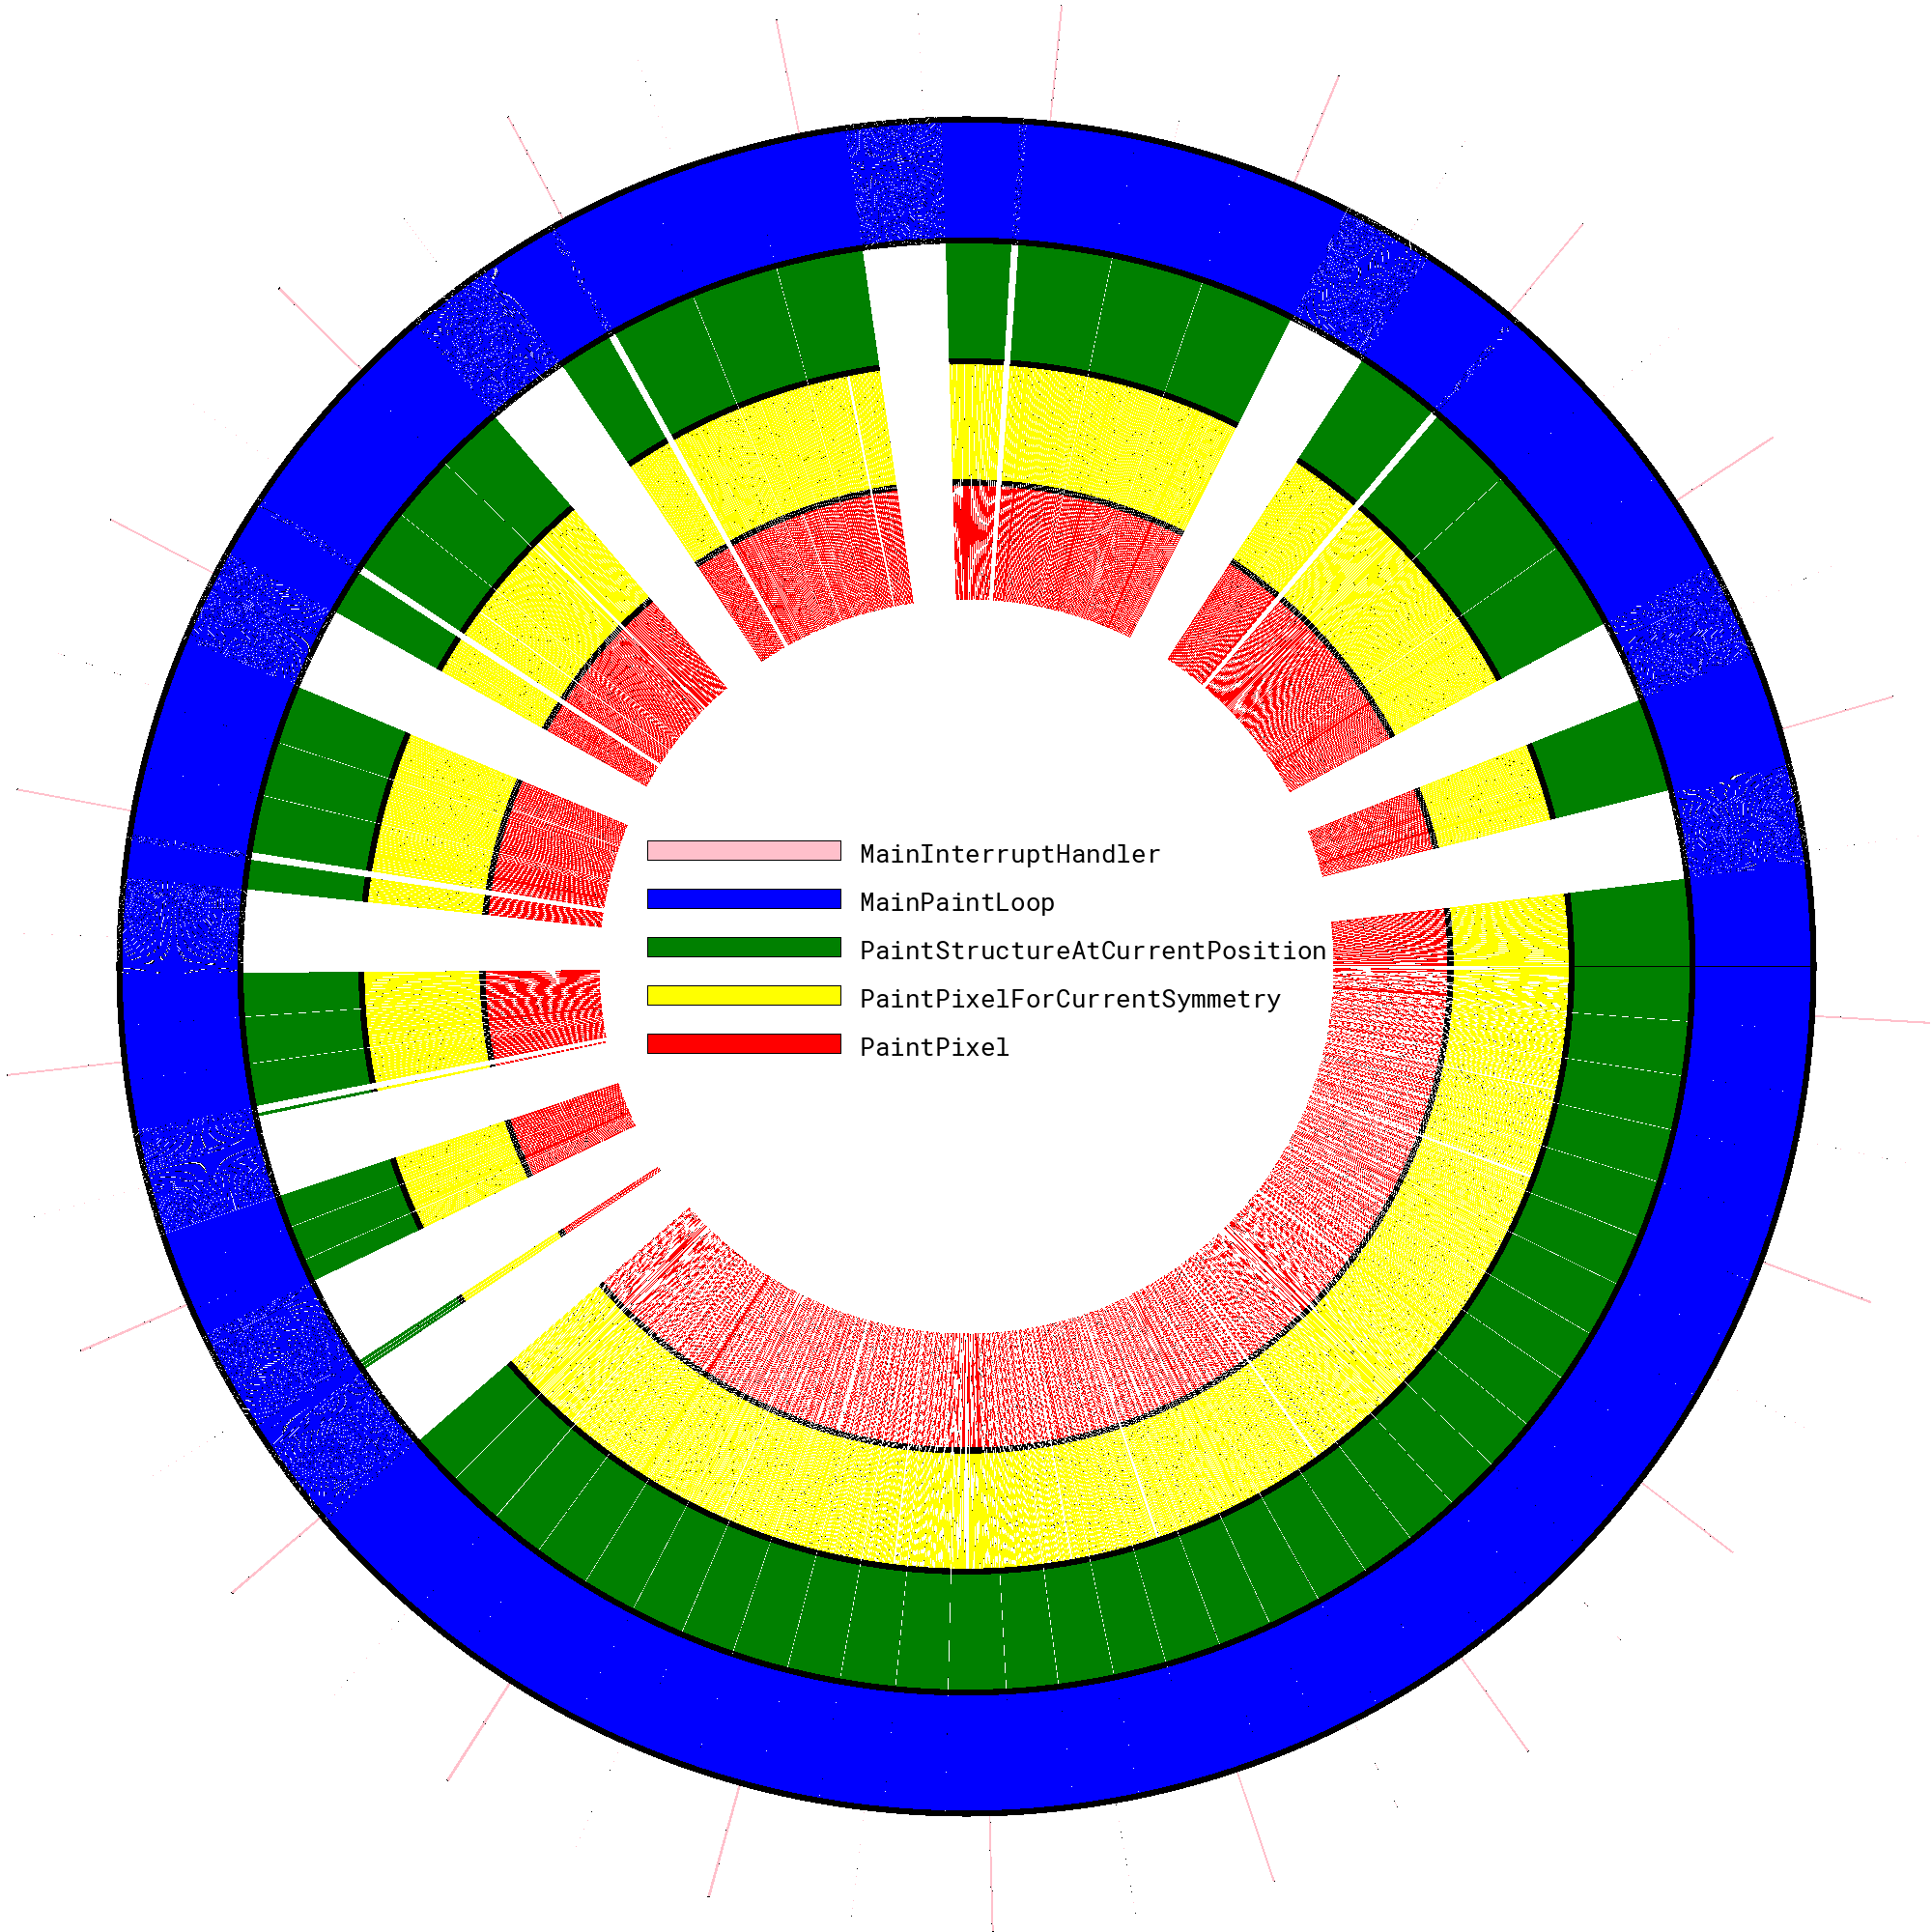
\includegraphics[width=10cm]{src/listing_commentary/execution_cycle_listing.png}%           
  \end{adjustbox}                                                        
\caption{The execution map of a full pattern evolution in the listing edition of Psychedelia.}                                           
\end{figure}                                                               
\clearpage
\begin{minipage}[b]{0.33\linewidth}
\begin{lrbox}{\mybox}%
\begin{lstlisting}[basicstyle=\ttfamily\tiny]
currentColorIndexArray   
 .BYTE $FF,$FF,$FF,$FF,$FF,$FF,$FF,$FF
 .BYTE $FF,$FF,$FF,$FF,$FF,$FF,$FF,$FF
 .BYTE $FF,$FF,$FF,$FF,$FF,$FF,$FF,$FF
 .BYTE $FF,$FF,$FF,$FF,$FF,$FF,$FF,$FF
 .BYTE $00,$00,$00,$00,$00,$00,$00,$00
 .BYTE $00,$00,$00,$00,$00,$00,$00,$00
 .BYTE $00,$00,$00,$00,$00,$00,$00,$00
 .BYTE $00,$00,$00,$00,$00,$00,$00,$00

initialFramesRemainingToNext   
 .BYTE $0C,$0C,$0C,$0C,$0C,$0C,$0C,$0C
 .BYTE $0C,$0C,$0C,$0C,$0C,$0C,$0C,$0C
 .BYTE $0C,$0C,$0C,$0C,$0C,$0C,$0C,$0C
 .BYTE $0C,$0C,$0C,$0C,$0C,$0C,$0C,$0C
 .BYTE $00,$00,$00,$00,$00,$00,$00,$00
 .BYTE $00,$00,$00,$00,$00,$00,$00,$00
 .BYTE $00,$00,$00,$00,$00,$00,$00,$00
 .BYTE $00,$00,$00,$00,$00,$00,$00,$00

framesRemainingToNextPaint   
 .BYTE $04,$07,$01,$02,$03,$06,$07,$06
 .BYTE $0C,$02,$03,$06,$07,$01,$02,$02
 .BYTE $04,$04,$07,$01,$02,$03,$06,$07
 .BYTE $0C,$02,$03,$02,$03,$07,$01,$02
 .BYTE $00,$00,$00,$00,$00,$00,$00,$00
 .BYTE $00,$00,$00,$00,$00,$00,$00,$00
 .BYTE $00,$00,$00,$00,$00,$00,$00,$00
 .BYTE $00,$00,$00,$00,$00,$00,$00,$00

;------------------------------
; ReinitializeSequences
;------------------------------
ReinitializeSequences   
 LDX #$00
 TXA 
b42D9   
 STA pixelXPositionArray,X
 STA pixelYPositionArray,X
 STA currentColorIndexArray,X
 STA initialFramesRemainingToNext,X
 STA framesRemainingToNextPaint,X
 INX 
 CPX #$40
 BNE b42D9
 RTS 

;------------------------------
; LaunchPsychedelia
;------------------------------
LaunchPsychedelia   
 JSR ReinitializeSequences
 JSR SetUpIntteruptHandlers

;------------------------------
; MainPaintLoop
;------------------------------
MainPaintLoop   
 INC currentIndexToPixelBuffers
 LDA currentIndexToPixelBuffers
 AND maskForFireOffset
 STA currentIndexToPixelBuffers
 TAX 
 DEC framesRemainingToNextPaint,X
 BNE GoBackToStartOfLoop

 LDA initialFramesRemainingToNext,X
 STA framesRemainingToNextPaint,X

 LDA currentColorIndexArray,X
 CMP #$FF
 BEQ GoBackToStartOfLoop

 STA colorIndexForCurrentPixel
 LDA pixelXPositionArray,X
 STA pixelXPosition
 LDA pixelYPositionArray,X
 STA pixelYPosition
 JSR PaintStructureAtCurrentPosition
 LDX currentIndexToPixelBuffers
 DEC currentColorIndexArray,X
GoBackToStartOfLoop   
 JMP MainPaintLoop

;------------------------------
; SetUpInterruptHandlers
;------------------------------
SetUpIntteruptHandlers   
 SEI 
 LDA #<MainInterruptHandler
 STA $0314    ;IRQ
 LDA #>MainInterruptHandler
 STA $0315    ;IRQ

 LDA #$0A
 STA cursorXPosition
 STA cursorYPosition

 LDA #$01
 STA $D015    ;Sprite display Enable
 STA $D027    ;Sprite 0 Color
 CLI 
 RTS 

\end{lstlisting}
\end{lrbox}%
\scalebox{0.8}{\usebox{\mybox}}
\end{minipage}
\hspace{-0.1cm}
\begin{minipage}[b]{0.33\linewidth}
\begin{lrbox}{\mybox}%
\begin{lstlisting}[basicstyle=\ttfamily\tiny]

currentIndexToPixelBuffers   .BYTE $08 
stepsToNextInputCheck 
 .BYTE $01
lastColorPainted
 .BYTE $00

;------------------------------
; MainInterruptHandler
;------------------------------
MainInterruptHandler   
 DEC stepsToNextInputCheck
 BEQ b4353
 JMP RETURN_FROM_INTERRUPT

b4353   LDA #$02
 STA stepsToNextInputCheck
 LDA #$00
 STA currentColorToPaint

 JSR PaintCursorAtCurrentPosition
 LDA $DC00    ;CIA1: Data Port Register A
 AND #$03
 CMP #$03
 BEQ CheckIfCursorMovedLeftOrRight

 CMP #$02
 BEQ PlayerHasPressedDown

 INC cursorYPosition
 INC cursorYPosition

PlayerHasPressedDown   
 DEC cursorYPosition
 LDA cursorYPosition
 CMP #$FF
 BNE CheckIfCursorAtBottom

 LDA #$17
 STA cursorYPosition
 JMP CheckIfCursorMovedLeftOrRight

CheckIfCursorAtBottom   
 CMP #NUM_ROWS
 BNE CheckIfCursorMovedLeftOrRight

 LDA #$00
 STA cursorYPosition

CheckIfCursorMovedLeftOrRight   
 LDA $DC00    ;CIA1: Data Port Register A
 AND #$0C
 CMP #$0C
 BEQ CheckIfPlayerPressedFire

 CMP #$08
 BEQ CursorMovedLeft

 ; Player has pressed right.
 INC cursorXPosition
 INC cursorXPosition

CursorMovedLeft   
 DEC cursorXPosition
 LDA cursorXPosition
 CMP #$FF
 BNE CheckIfCursorAtExtremeRight

 LDA #$27
 STA cursorXPosition
 JMP CheckIfPlayerPressedFire

CheckIfCursorAtExtremeRight   
 CMP #NUM_COLS
 BNE CheckIfPlayerPressedFire
 LDA #$00
 STA cursorXPosition

CheckIfPlayerPressedFire   
 LDA $DC00    ;CIA1: Data Port Register A
 AND #$10
 BEQ PlayerHasntPressedFire

 ; Player has pressed fire.
 LDA #$00
 STA stepsSincePressedFire
 JMP DrawCursorAndReturnFromInterrupt

PlayerHasntPressedFire   
 LDA stepsExceeded255
 BEQ b43D7
 LDA stepsSincePressedFire
 BNE DrawCursorAndReturnFromInterrupt

 INC stepsSincePressedFire
b43D7
 INC seedValueForArrayIndices
 LDA seedValueForArrayIndices
 AND maskForFireOffset
 STA seedValueForArrayIndices

\end{lstlisting}
\end{lrbox}%
\scalebox{0.8}{\usebox{\mybox}}
\end{minipage}
\hspace{-0.1cm}
\begin{minipage}[b]{0.33\linewidth}
\begin{lrbox}{\mybox}%
\begin{lstlisting}[basicstyle=\ttfamily\tiny]
UpdateColorIndexArray  
 TAX 
 LDA currentColorIndexArray,X
 CMP #$FF
 BNE DrawCursorAndReturnFromInterrupt

 LDA cursorXPosition
 STA pixelXPositionArray,X
 LDA cursorYPosition
 STA pixelYPositionArray,X
 LDA #COLOR_MAX
 STA currentColorIndexArray,X

 LDA smoothingDelay
 STA initialFramesRemainingToNext,X
 STA framesRemainingToNextPaint,X

DrawCursorAndReturnFromInterrupt   
 JSR LoadXAndYOfCursorPosition
 LDA (curCursorLineColorRamLoPtr),Y
 AND #COLOR_MAX
 STA lastColorPainted
 LDA #WHITE
 STA currentColorToPaint
 JSR PaintCursorAtCurrentPosition
 JMP RETURN_FROM_INTERRUPT

;------------------------------
; LoadXAndYOfCursorPosition
;------------------------------
LoadXAndYOfCursorPosition   
 LDX cursorYPosition
 LDA colorRAMLineTableLoPtrArray,X
 STA curCursorLineColorRamLoPtr
 LDA colorRAMLineTableHiPtrArray,X
 STA curCursorLineColorRamHiPtr
 LDY cursorXPosition
 RTS 

;------------------------------
; PaintCursorAtCurrentPosition
;------------------------------
PaintCursorAtCurrentPosition   
 JSR LoadXAndYOfCursorPosition
 LDA currentColorToPaint
 STA (curCursorLineColorRamLoPtr),Y
 RTS 

cursorXPosition        .BYTE $1E
cursorYPosition        .BYTE $0D
seedValueForArrayIndices .BYTE $1A
maskForFireOffset      .BYTE $1F
stepsSincePressedFire  .BYTE $00
stepsExceeded255       .BYTE $00
smoothingDelay         .BYTE $0C
 .BYTE $00,$00,$00,$00,$00,$00,$00
 .BYTE $5B,$00,$00,$00,$00,$00,$00,$00
 .BYTE $00,$00,$00,$00,$00,$00,$00,$00
 .BYTE $00,$00,$00,$00,$00,$00,$00,$00
 .BYTE $00,$00,$00,$00,$00,$00,$00,$00
 .BYTE $00,$00,$00,$00,$00,$00,$00,$00
 .BYTE $FF,$00,$00,$00,$00,$00,$00,$00
 .BYTE $00,$00,$00,$00,$00,$00,$00,$00
 .BYTE $00,$00,$00,$00,$00,$00,$00,$00
 .BYTE $00,$00,$00,$00,$00,$00,$00,$00
 .BYTE $00,$00,$00,$00,$00,$00,$00,$00
 .BYTE $00,$00,$00,$00,$00,$00,$00,$00
 .BYTE $00,$00,$00,$00,$00,$00,$00,$00
 .BYTE $00,$00,$00,$00,$00,$00,$00,$00
 .BYTE $00,$00,$00,$00,$00,$00,$00,$00
 .BYTE $00,$00,$00,$00,$00,$00,$00,$00
 .BYTE $00,$00,$00,$00,$00,$00,$00,$00
 .BYTE $00,$00,$00,$00,$00,$00,$00,$00
 .BYTE $00,$00,$00,$00,$00,$00,$00,$00
 .BYTE $00,$00,$00,$00,$00,$00,$00,$00
 .BYTE $00,$00,$00,$00,$00,$00,$00,$00
 .BYTE $00,$00,$00,$00,$00,$00,$00,$00
 .BYTE $00,$00,$00,$00,$00,$00,$00,$00
 .BYTE $00,$00,$00,$00,$00,$00,$00,$00
 .BYTE $00,$00,$00,$00,$00,$00,$00

bannerText   
 .TEXT $00,"PSYCHEDELIA...A FORETASTE BY JEFF MINTER"

;------------------------------
; InitializeScreenAndText
;------------------------------
InitializeScreenAndText   
 JSR InitializeScreen

 LDX #NUM_COLS
_Loop   LDA bannerText,X
 STA SCREEN_RAM + $03BF,X
 LDA #$0C
 STA COLOR_RAM + $03BF,X
 DEX 
 BNE _Loop
 RTS 

 .BYTE $00,$00,$00,$BF,$00,$9D,$00,$FF
 .BYTE $00,$FF,$00,$FF,$00,$FF,$00,$DF
 .BYTE $FF,$FF,$FF,$FF,$00

\end{lstlisting}
\end{lrbox}%
\scalebox{0.8}{\usebox{\mybox}}
\end{minipage}
\clearpage
\textbf{Lines 401-720. } This second half of the program contains, towards the bottom of the first column
opposite, the main loop (\icode{MainPaintLoop}) that
runs round and round in a circle for as long as the program itself is running. 

The bulk of the rest of the listing
is what we call an 'interrupt handler', a routine that gets called numerous times every second by the C64
and so is a useful place to do things like checking for user input on the keyboard or joystick, which
is precisely what \icode{MainInterruptHandler} in fact does.

Towards the end, in the third column, we find a couple of helper functions tagged on: \icode{LoadXAndYOfCursorPosition}
and \icode{PaintCursorAtCurrentPosition}. These are used by the interrupt handler so can be considered part
of the interrupt handler itself. 

The very last part contains some variables used by the handler, e.g \icode{cursorXPosition} and \icode{cursorYPosition}.
And then a longish section of unused data, just zero bytes, followed by the text storage for the program's title
screen. We encountered this part in our first chapter, where we saw how the magazine listing had been misprinted
at this point and left us attempting to piece it back together with the program's title as a useful clue for the
missing bytes.

And that is it - a quite tiny program that fits (not quite legibly I'll admit) on just two pages. In the rest of
this chapter we'll dig into the details of each of these routines. It may be useful to refer back here every now
and then to get a sense of where you are on the map as we pull apart the detail.

\clearpage

